%-------------------------------------------------------------------------------
%	NAME:	report.tex
%	AUTHOR: Connor Beardsmore - 15504319
%	LAST MOD:	28/09/17
%	PURPOSE:	FCC Assignment Report
%	REQUIRES:	NONE
%-------------------------------------------------------------------------------

\documentclass[]{article}
\usepackage[ margin=3cm ]{geometry}
\usepackage{graphicx}
\usepackage{fancyhdr}
\usepackage{float}
\usepackage{hyperref}
\usepackage{transparent}
\usepackage{multicol}
\usepackage{amsmath}
\usepackage[final]{pdfpages}
\usepackage{listings}
\usepackage{color}
\usepackage{algorithmicx}
\usepackage{algpseudocode}
\usepackage{amssymb}
\usepackage[style=chicago-authordate,backend=biber]{biblatex}

\pagestyle{fancy}
\fancyhf{}
\lhead{Connor Beardsmore - 15504319}
\rhead{FCC200}
\lfoot{April 2017}
\rfoot{\thepage}

\pagenumbering{arabic}
\graphicspath{{./images/}}

\addbibresource{bib/references.bib}
\nocite{*}

%-------------------------------------------------------------------------------
% CODE HIGHLIGHTING FOR LISTINGS
\definecolor{codegreen}{rgb}{0,0.6,0}
\definecolor{codegray}{rgb}{0.5,0.5,0.5}
\definecolor{codepurple}{rgb}{0.58,0,0.82}
\definecolor{backcolour}{rgb}{0.99,0.99,0.99}

\lstdefinestyle{mystyle}{
	backgroundcolor=\color{backcolour},   
	commentstyle=\color{codegreen},
	keywordstyle=\color{magenta},
	numberstyle=\tiny\color{codegray},
	stringstyle=\color{codepurple},
	basicstyle=\footnotesize,
	breakatwhitespace=false,         
	breaklines=true,                 
	captionpos=b,                    
	keepspaces=true,                 
	numbers=left,                    
	numbersep=5pt,                  
	showspaces=false,                
	showstringspaces=false,
	showtabs=false,                  
	tabsize=2
}

\lstset{style=mystyle}


%-------------------------------------------------------------------------------
\begin{document}
%-------------------------------------------------------------------------------
% TITLE PAGE

\begin{titlepage}
	\begin{center}
		\vspace*{1cm}
		\LARGE\textbf{FCC200 Report}
		\break
		Affine Cipher and S-DES Implementation
		\vspace{1cm}
		\break
		\Large\textbf{Connor Beardsmore - 15504319} 
		\vspace{15cm}

		\normalsize
		Curtin University \\
		Science and Engineering \\
		Perth, Australia \\
	    April 2017
	    
	\end{center}
\end{titlepage}

%-------------------------------------------------------------------------------
% AFFINE CIPHER

\vspace*{-0.8cm}
\begin{center}
	\section*{Affine Cipher}
\end{center}

\vspace*{0.8cm}
\subsection*{Compute Eligible Keys}

There are two keys required, \textit{a} and \textit{b}. The first is required to be \textit{coprime} with the length of the alphabet, in this scenario \textit{26}. The second key representing the linear shift must be both positive and less than the length of the alphabet. To check if the \textit{a} value is coprime, the following greatest common denominator check was utilized. If the greatest common denominator of \textit{a} and 26 is 1, the value of \textit{a} is \textit{coprime} and the key is valid in combination with any valid \textit{b} value.\\

\lstinputlisting[language=C,linerange={34-60} ]{../affine/keyeligible.c} 

\vspace{0.5cm}
The results of calling this function on all \textit{a} values from 1 to 25 are as follows:\\

\begin{multicols}{2}
	\begin{itemize}
		\item \textbf{gcdFunction( 1, 26 ) = 1}
		\item gcdFunction( 2, 26 ) = 2
		\item \textbf{gcdFunction( 3, 26 ) = 1}
		\item gcdFunction( 4, 26 ) = 2
		\item \textbf{gcdFunction( 5, 26 ) = 1}
		\item gcdFunction( 6, 26 ) = 2
		\item \textbf{gcdFunction( 7, 26 ) = 1}
		\item gcdFunction( 8, 26 ) = 2
	    \item \textbf{gcdFunction( 9, 26 ) = 1}
		\item gcdFunction( 10, 26 ) = 2
		\item \textbf{gcdFunction( 11, 26 ) = 1}
		\item gcdFunction( 12, 26 ) = 2
		\item gcdFunction( 13, 26 ) = 13
		\item gcdFunction( 14, 26 ) = 2
		\item \textbf{gcdFunction( 15, 26 ) = 1}
		\item gcdFunction( 16, 26 ) = 2
		\item \textbf{gcdFunction( 17, 26 ) = 1}
		\item gcdFunction( 18, 26 ) = 2
		\item \textbf{gcdFunction( 19, 26 ) = 1}
		\item gcdFunction( 20, 26 ) = 2
		\item \textbf{gcdFunction( 21, 26 ) = 1}
		\item gcdFunction( 22, 26 ) = 2	
		\item \textbf{gcdFunction( 23, 26 ) = 1}
		\item gcdFunction( 24, 26 ) = 2
		\item \textbf{gcdFunction( 25, 26 ) = 1}
	\end{itemize}
\end{multicols}


\vspace{0.5cm}

The full list of valid \textit{a} values is: \textbf{1, 3, 5, 7, 9, 11, 15, 17, 19, 21, 23, 25}\\

The full list of valid \textit{b} values is: \textbf{0 to 25 inclusive}\\

There are a total of 12 possible \textit{a} values that are coprime with \textit{26}. Each of these values can have a shift value (\textit{b}) of 0 to 25. Thus, the total number of eligible keys is:

$$12*26=312$$

Of these, 26 keys are trivial Caesar ciphers and 286 are non-trivial (\cite{maintext}).
\newpage
\subsection*{Recovered Plaintext}

The implemented Affine cipher works correctly with all eligible keys. The recovered plaintext in Figure 3 is identical to the original plaintext of Figure 1. No major problems were encountered during the implementation phase.
\vspace{1cm}
\begin{figure}[H]
	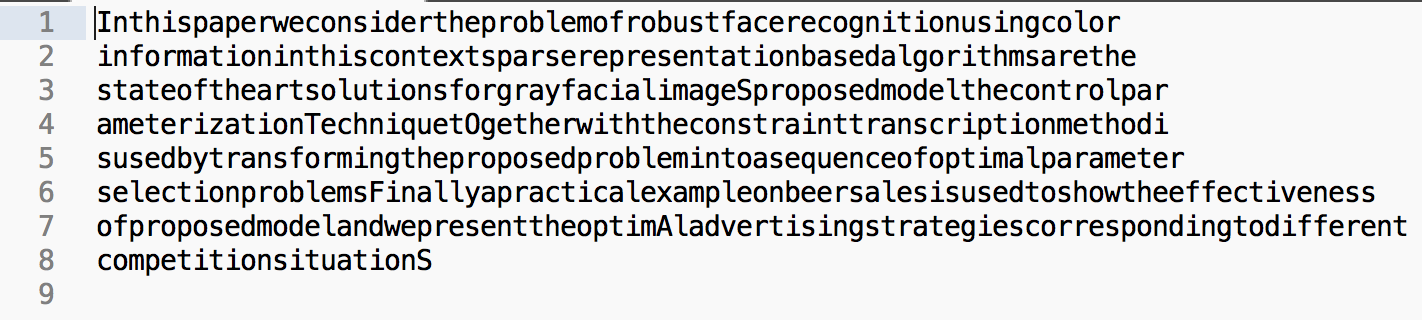
\includegraphics[width=\textwidth]{affine_plaintext.png}
	\caption{Original Plaintext}
	\centering
\end{figure}

\begin{figure}[H]
	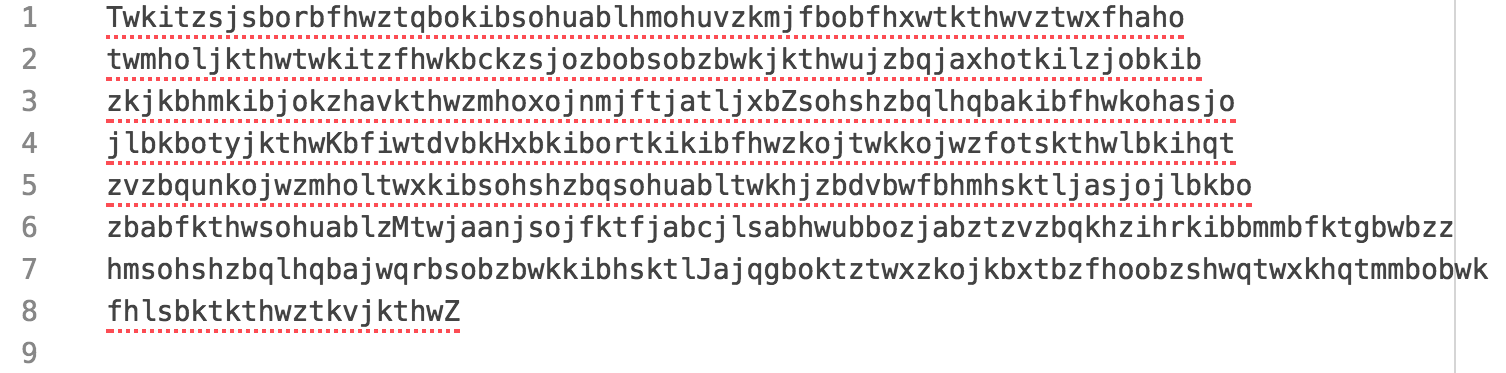
\includegraphics[width=\textwidth]{affine_ciphertext.png}
	\caption{Encrypted Ciphertext}
	\centering
\end{figure}

\begin{figure}[H]
	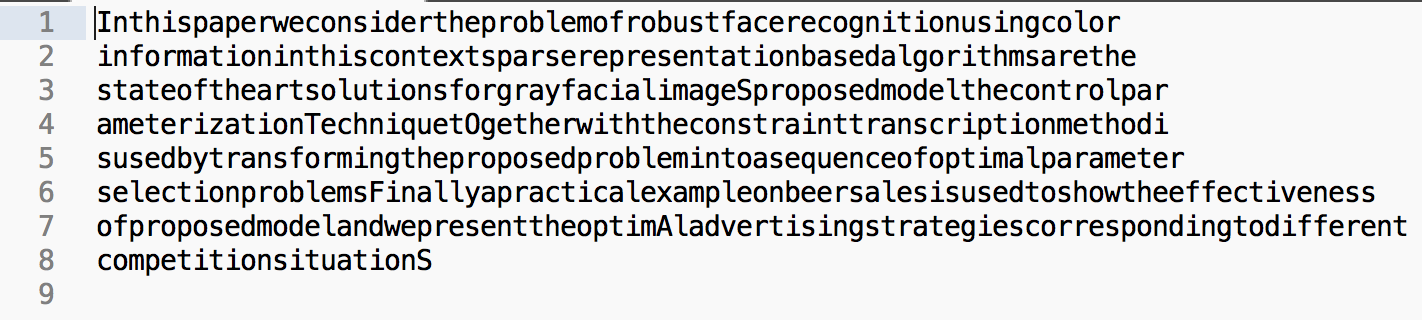
\includegraphics[width=\textwidth]{affine_plaintext.png}
	\caption{Recovered Plaintext}
	\centering
\end{figure}

\newpage
\subsection*{Affine Mathematical Proof}

The encryption and decryption functions for the affine cipher are as follows:

$$E(x)=c=(ax+b)\;mod\;m$$

$$D(x)=x=a^{-1}(c-b)\;mod\;m$$

where:

$$x = plaintext$$
$$c = ciphertext$$
$$m = alphabet\;length$$
$$a,b=keys$$
\vspace{0.5cm}

The modular multiplicative inverse of \textit{a} - \textit{a\textsuperscript{-1}} -  is defined as:

$$1=aa^{-1}\;mod\;m$$

It can be shown that \textit{D(x)} is the inverse of \textit{E(x)} via the modular arithmetic laws:

\begin{equation*}
\begin{split}
D(E(x)) & = a^{-1}(E(x)-b)\;mod\;m \\
& = a^{-1}(( (ax+b)\;mod\;m )-b)\;mod\;m \\
& = a^{-1} (ax+b-b) \;mod\;m \\
& = a^{-1}ax\;mod\;m \\
& = x\;mod\;m
\end{split}
\end{equation*}

\newpage
\subsection*{Letter Distribution}

For the given test file shown in Figure 2, the following values and Figure 4 illustrate the letter distribution and relative frequencies. The breakdown of the relative frequencies allow for cryptanalysis to be performed on the affine cipher, thus leading to a factor in its lack of security.

\begin{multicols}{7}
	\begin{itemize}
		\item A: 35
		\item B: 7
		\item C: 17
		\item D: 14
		\item E: 65
		\item F: 14
		\item G: 10
		\item H: 16
		\item I: 41
		\item J: 0
		\item K: 0
		\item L: 18
		\item M: 16
		\item N: 35
		\item O: 50
		\item P: 23
		\item Q: 2
		\item R: 39
		\item S: 39
		\item T: 53
		\item U: 8
		\item V: 2
		\item W: 4
		\item X: 2
		\item Y: 3
		\item Z: 1
	\end{itemize}
\end{multicols}

\begin{figure}[H]
	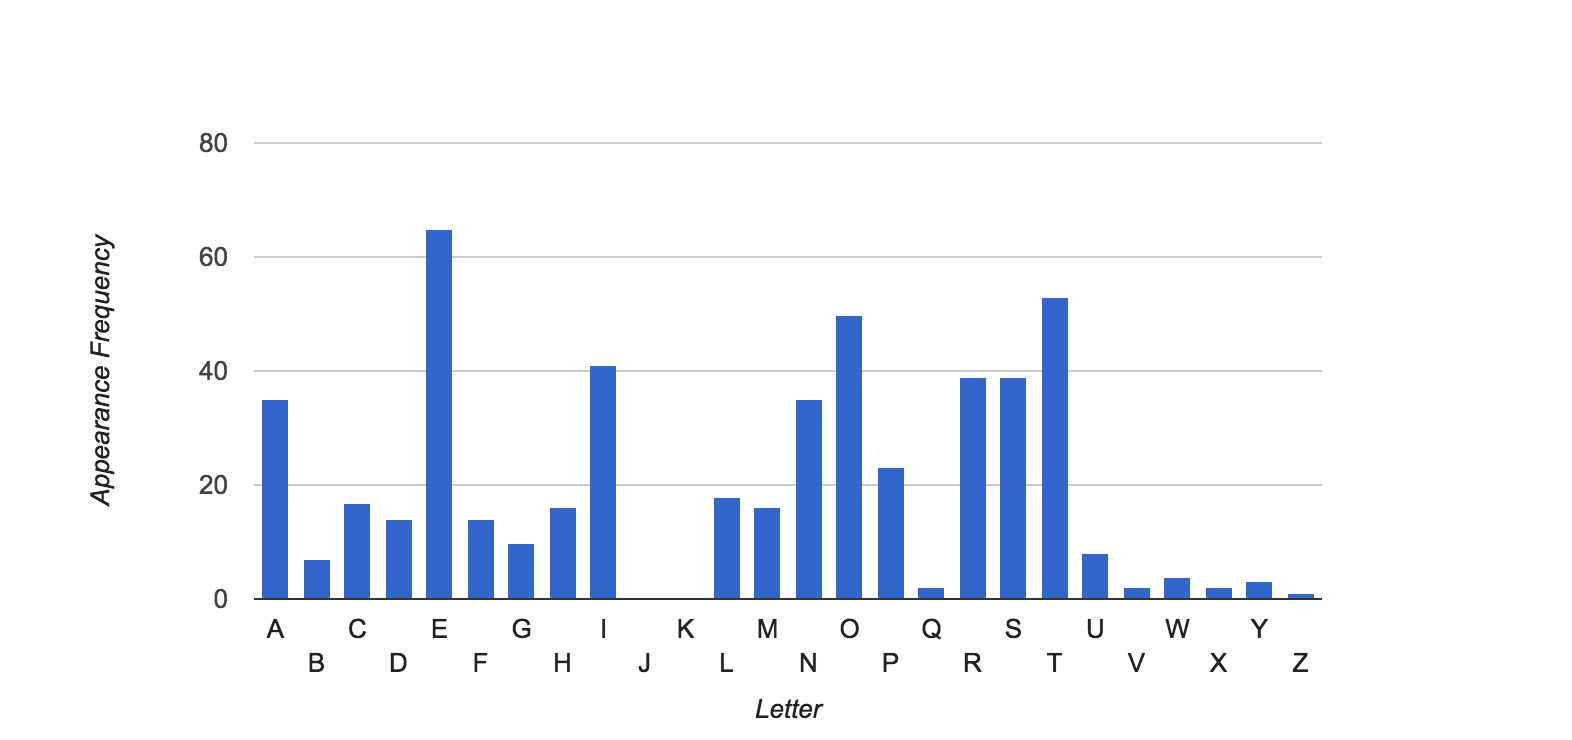
\includegraphics[width=18cm]{frequency.png}
	\caption{Letter Distributions}
	\centering
\end{figure}

\break
%-------------------------------------------------------------------------------
% S-DES ENCRYPTION

\vspace*{-0.8cm}
\begin{center}
	\section*{S-DES}
\end{center}

\vspace*{0.8cm}
\subsection*{S-DES Mathematical Proof}

Let the following definitions apply:

$$m = 8bit\;plaintext$$
$$c = 8bit\;ciphertext$$
$$k = 10bit\;key$$
$$IP = initial\;permutation$$
$$IP^{-1} = inverse\;of\;initial\;permutation$$

$$L_i = left\;block\;of\;m\;(5bit)$$
$$R_i = right\;block\;of\;m\;(5bit)$$\\

Let encryption be defined as the following set of three steps:\\

\begin{center}
\textbf{Step 1}
$$(L_0,R_0)=IP(p)$$

\textbf{Step 2}
$$Let\;i=1,2$$
$$Let\;k_i=subkey\;i\;(8bit)$$
$$L_i=R_{i-1}$$
$$R_i=L_{i-1}\oplus F(R_{i-1},k_i)$$

\textbf{Step 3}
$$c=IP^{-1}(L_{16},R_{16})$$
\end{center}

Next, it can be proven that plaintext \textit{m} can be discovered from ciphertext \textit{c} given the full key \textit{k}:

$$c=IP^{-1}(L_{16},R_{16})$$


\newpage
\subsection*{Pseudo Code Structure}

The pseudo-code structure of the three key functions utilized in the S-DES implementation is illustrated below. The three function constitute the core functionality of the S-DES algorithm.\\

\begin{algorithmic}
\Function{KeyGeneration}{int key}
	\State $key\gets $ \Call{permute}{ key, P10 }
	\State \Call{leftshift}{ key, 1 }
	\State $subkeys[0]\gets $ \Call{permute}{ key, P8 }
	\State \Call{leftshift}{ key, 2 }
	\State $subkeys[1]\gets $ \Call{permute}{ key, P8 }
	\State \Return subkeys
\EndFunction
\end{algorithmic}


\vspace{0.5cm}

\begin{algorithmic}
	\Function{SwitchFunction}{int input}
		\State $ right \gets bits \;\&\&\; ( ( 1 << 4 ) - 1 ) $
		\State $ left \gets bits >>> 4 $
		\State $ output \gets left \;||\; ( right << 4 )$
		\State \Return output
	\EndFunction
\end{algorithmic}

\vspace{0.5cm}

\begin{algorithmic}
	\Function{FeistalKeyRound}{int message, int subkey}
	
	\State $halves\gets $ \Call{split}{ message }
	\State $fMap \gets $ \Call{fMapping}{ rightHalf, subkey }	
	\State $ leftHalf \gets leftHalf \oplus fMap $
	\State \Return combined $ leftHalf + rightHalf $
	\EndFunction
\end{algorithmic}

\vspace{0.5cm}
\noindent
For clarity, the pseudo code structure for the fMap function in addition to how the above three functions are combined for encryption is covered below.
\vspace{0.5cm}
\begin{algorithmic}
	\Function{FMapping}{ int message, int subkey}
	
	\State $message\gets $ \Call{permute}{ message, EP }
	\State $ message \gets message \oplus subkey $
	\State $ message \gets $ \Call{sbox\_calculation}{message}	
	\State $message\gets $ \Call{permute}{ message, P4 }	
	\State \Return $message$
	\EndFunction
\end{algorithmic}

\vspace{0.5cm}
\begin{algorithmic}
	\Function{Encryption}{ int message, int[] subkey}
	
	\State $message\gets $ \Call{permute}{ message, IP }
	\State $message\gets $ \Call{feistalRound}{ message, subkey[0] }
	\State \Call{switchFunction}{message}	
	\State $message\gets $ \Call{feistalRound}{ message, subkey[1] }	
	\State $message\gets $ \Call{permute}{ message, IP\_INVERSE }
	\State \Return $message$
	\EndFunction
\end{algorithmic}

\newpage
\subsection*{Encrypted Test File}

The included code implementation for S-DES works correctly and there were no difficulties faced in the process of programming.

\begin{figure}[H]
	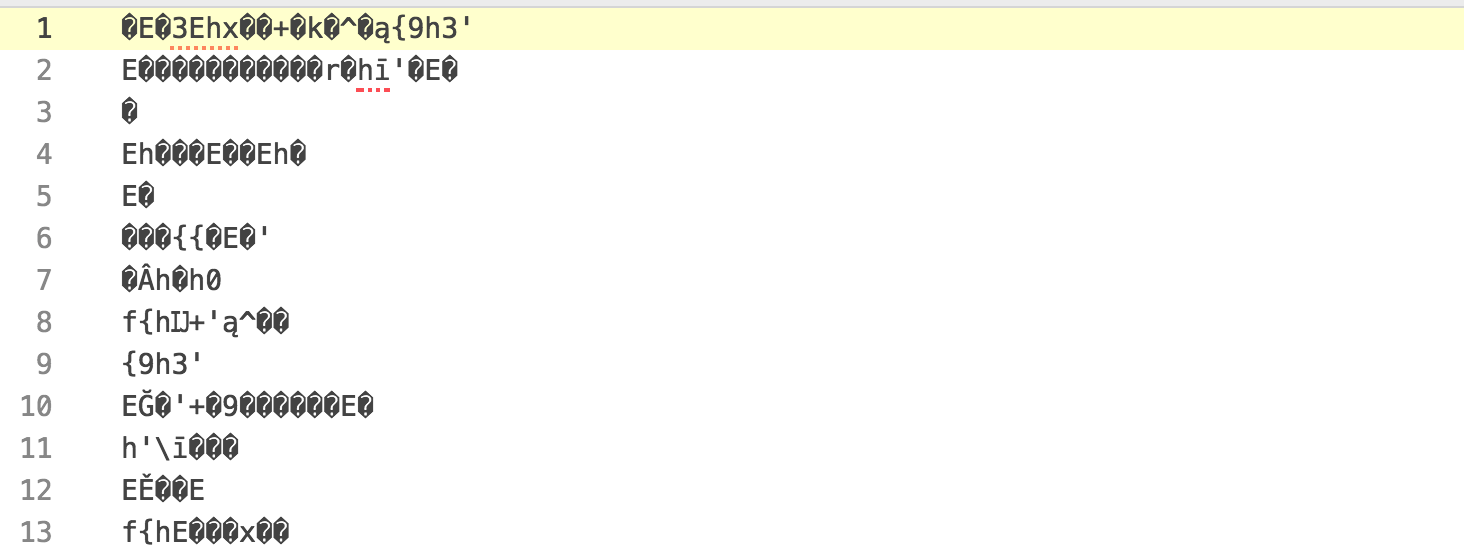
\includegraphics[height=\textheight/6,width=\textwidth]{sdes_cipher1.png}
	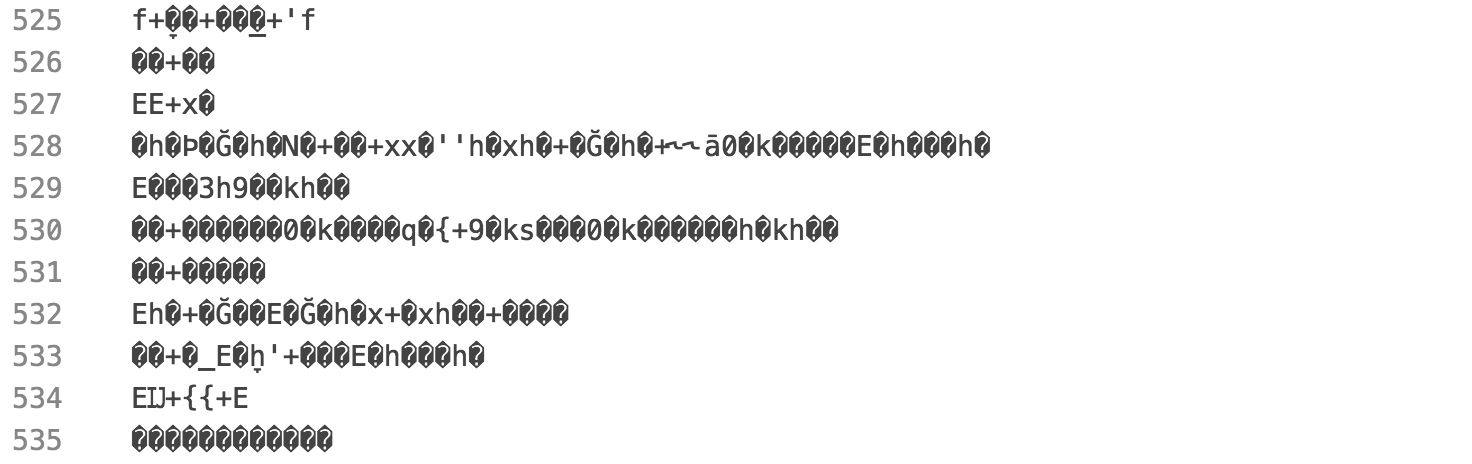
\includegraphics[height=\textheight/6,width=\textwidth]{sdes_cipher2.png}	
	\caption{S-DES Cipher Text}
	\centering
\end{figure}

\vspace{0.5cm}
\subsection*{Decrypted Test File}

\begin{figure}[H]
	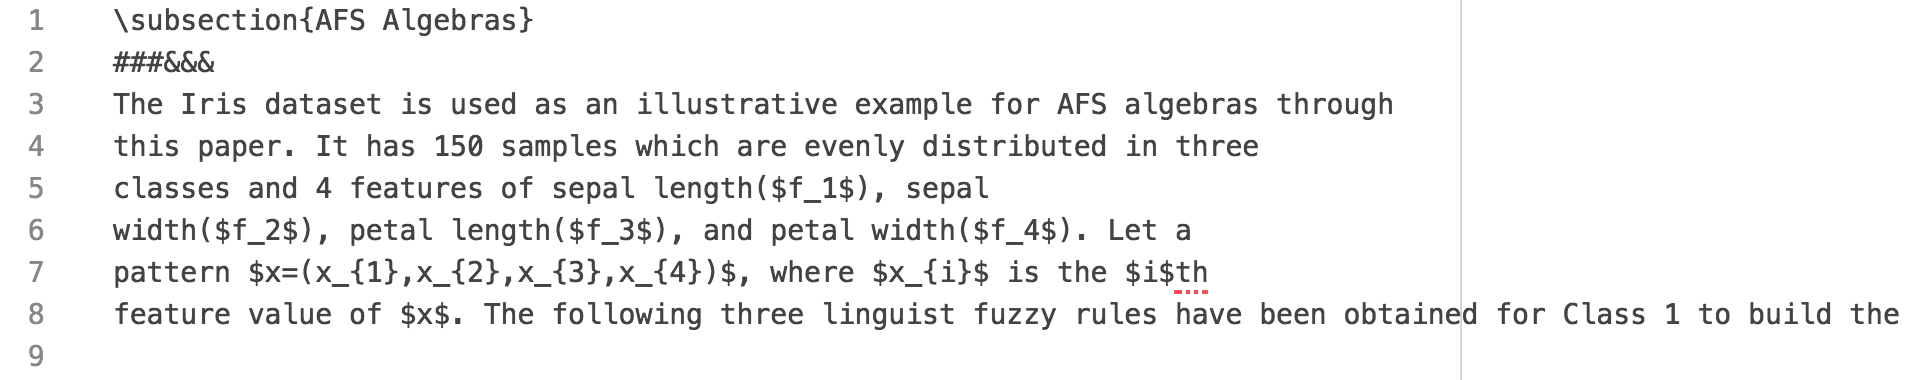
\includegraphics[width=\textwidth]{sdes_plain1.png}
	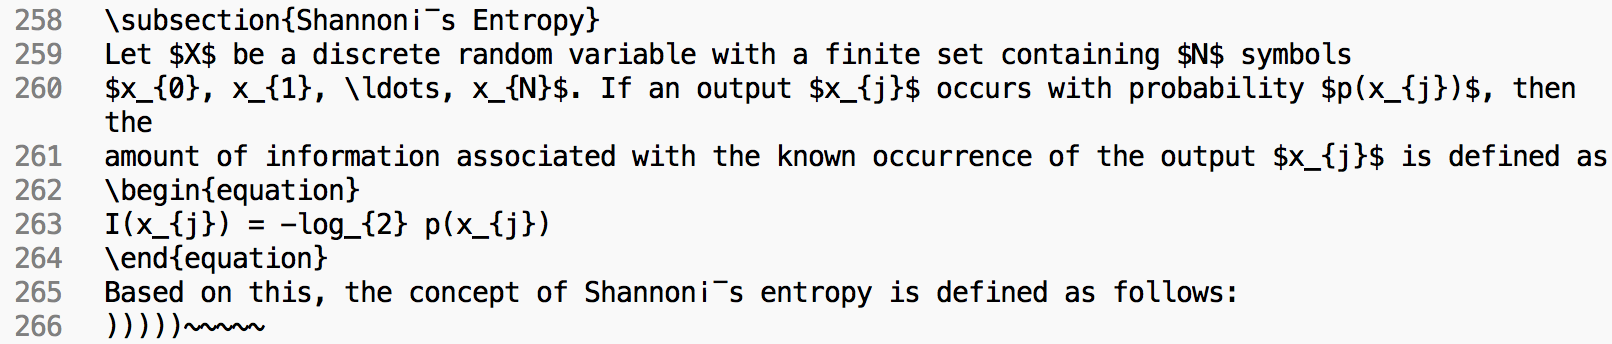
\includegraphics[width=\textwidth]{sdes_plain2.png}	
	\caption{S-DES Plain Text}
	\centering
\end{figure}

\newpage
\subsection*{Utilization of an all 1 Key}

Performing encryption and decryption with S-DES utilizing a key of all 1's (11111111) does not significantly alter how the algorithm performs. However, during the two feistal key rounds, the subkeys will be equivalent. The S-DES algorithm is symmetric, with the difference between encryption and decryption being the different subkeys utilized in the two rounds. If the subkeys are identical, both encryption and decryption end up being the same process. Thus in this situation, both the following apply:

$$x=E( E(x) )$$

$$x=D( D(x) )$$

The same situation will occur with a key of all 0's (0000000000) or a key of alternating 1's and 0's (1010101010) for the same reasons. These keys are termed "weak keys" (\cite{alttext}). Due to the large keyspace of S-DES, the rare occurence of these weak keys is not considered a major flaw in the overriding algorithm.

\subsection*{Modify S-Boxes}


The S-BOX values in the SDESConstants.java file were modified to ensure that the S-DES algorithm still performs accurately. Modification of the S-BOX values within the given constraints - each row must contains 0, 1, 2 and 3 - did not affect the overall algorithm. However, modification of the S-BOX values can reduce the security of DES significantly (\cite{maintext}).

\break
%-------------------------------------------------------------------------------
% FINAL QUESTIONS

\vspace*{-0.8cm}
\begin{center}
	\section*{Additional Questions}
\end{center}

\vspace*{0.8cm}
\subsection*{Threats}

wtf does this mean? security or transmission threats???

\subsection*{Source Coding}

Source coding in information transmission aims to compress natural messages for highly efficient message transfer.

\subsection*{Error Coding}

Error coding in information transmission attempts to enable a high information rate by the introduction of redundancy to data, as well as via error detection and correction mechanisms. A simplistic example of error coding is the repetition code. Forms of error detection and correction mechanisms include parity checksums in addition to the ISBN and UPC codes.

\subsection*{S-DES Coding}

The source coding in the S-DES implementation involves converting the plaintext ascii key into a 10-bit binary code. This is done by taking the hash code of the initial String and performing chopping to ensure a maximum 10-bit key. The implementation shown reads each byte individually from the file and thus no source coding was required. However if the file was read as ascii characters, the conversion of this into a binary representation would be a form of source coding.\\

The S-DES algorithm does not contain any error coding. No checkbits or replication bits are included to help detect errors. This is in contrast to the standard DES algorithm, where 8-bits of the 64-bit key are odd parity checksums. This implies that S-DES has a higher information rate than DES, at the cost of the possible detection of transmission errors (\cite{alttext}).

\subsection*{S-DES Confusion and Diffusion}

In S-DES, confusion is provided by the S-BOX substitutions performed within the feistal key round. Diffusion in contrast is provided by the permutations applied to the data included the expansion permutation utilized.

\pagebreak

%-------------------------------------------------------------------------------
% AFFINE CODE

\vspace*{-0.8cm}
\begin{center}
	\section*{Affine Source Code}
\end{center}

\subsection*{keyeligible.h}
\lstinputlisting[language=C,linerange={} ]{../affine/keyeligible.h}\pagebreak{}
\subsection*{keyeligible.c}
\lstinputlisting[language=C,linerange={} ]{../affine/keyeligible.c}\pagebreak{}
\subsection*{affine.h}
\lstinputlisting[language=C,linerange={} ]{../affine/affine.h}\pagebreak{}
\subsection*{affine.c}
\lstinputlisting[language=C,linerange={} ]{../affine/affine.c}\pagebreak{}

%-------------------------------------------------------------------------------
% SDES CODE

\vspace*{-0.8cm}
%\begin{center}
	\section*{S-DES Source Code}
%\end{center}

\subsection*{SDESConstants.java}
\lstinputlisting[language=java,linerange={} ]{../SDES/SDESConstants.java}\pagebreak{}
\subsection*{SDESBits.java}
\lstinputlisting[language=java,linerange={} ]{../SDES/SDESBits.java}\pagebreak{}
\subsection*{SDES.java}
\lstinputlisting[language=java,linerange={} ]{../SDES/SDES.java}\pagebreak{}

%-------------------------------------------------------------------------------   
% REFERENCES

\break
\setlength\bibitemsep{4\itemsep}
\printbibliography[heading=bibintoc,title={References}]

%-------------------------------------------------------------------------------
\end{document}   
%-------------------------------------------------------------------------------: